\section{Discussion}

\subsection{Implications for latent world model evaluation}

The failed repairs in Section~6 yield a clear evaluation implication. Endpoint metrics should not be the sole evaluation criterion for latent world models that use CEM-style planning. They test whether the representation carries task information; they do not test whether the planner can exploit that information during iterative search.

This distinction matters because CEM changes the distribution being evaluated. Endpoint ranking is computed on a fixed benchmark set, whereas planning uses proposal distributions shaped by previous elite selections. The final action comes from the last candidate pool, not from the endpoint set.

We therefore recommend a minimal planning-compatible reporting protocol: $\Rendpoint$ on a fixed endpoint set, $\Rpool$ on planner-produced candidate pools, and selection metrics for the executed action, including $M_\mathrm{rank1}$ and selection regret. This adds little overhead: it requires saving the final pool of CEM and scoring it with the physical cost already used during evaluation.

% REVISION: addresses W5
The three-level reporting protocol uses $C_\mathrm{real\_state}$ to compute $\Rpool$ and selection regret, so the full diagnostic is an evaluation-time audit rather than a deployable monitor. We therefore tested whether privilege-free quantities available from the learned cost alone predict high-regret pairs. The strongest global proxy was the standard deviation of the learned cost among the top-30 final-pool candidates, which correlated with selection regret at Spearman $\rho=0.314$ ($p=0.001$). Within the invisible-quadrant subset, the full-pool learned-cost spread was stronger, with $\rho=0.588$ ($p=0.017$). As a cross-check, learned-cost spread tracked privileged physical spread: $\rho(\mathrm{std}(\Cmodel), \mathrm{std}(C_\mathrm{real\_state}))=0.482$ ($p<0.001$). These proxies are not replacements for the full audit, but they show that partial monitoring is possible without simulator access. In particular, low learned-cost diversity in the final pool can flag candidate-pool compression and elevated selection risk.

\subsection{Intervention paths motivated by the framework}

The diagnostic framework also points to low-overhead future work. One direction is pool-aware termination, which would stop CEM when candidate diversity or elite-cost spread stagnates. Cost regularization could maintain elite spread during proposal updates. Adaptive projection scheduling could use simpler costs early and full-dimensional precision later. These directions treat the CEM pool as an object to monitor and shape, not as an invisible byproduct of endpoint geometry.

Section~\ref{sec:warp_ensemble} sharpens this point. Pool-level ranking labels provide strong corrective signal on seen pools, but the learned calibration does not transfer across held-out start-goal configurations. Future work should therefore move upstream to training-time approaches that enforce local isometry inside the encoder itself, such as contrastive regularization on simulated CEM pools or adversarial latent-space calibration.

% REVISION: addresses W4
\subsection{Optimizer dependence: CEM versus MPPI}
\label{sec:mppi}

We also tested whether endpoint-planning decoupling is specific to CEM's hard elite truncation. On 30 PushT pairs with three seeds per pair, we replaced the CEM update with an MPPI-style soft weighting update over all 300 candidates, using the same model, action parameterization, horizon, and terminal latent cost. MPPI achieved lower rank-1 planning success than CEM in this fixed-budget comparison (38.9\% versus 53.3\%), consistent with slower convergence under 30 iterations. However, the pool geometry gives the relevant diagnostic. MPPI preserved substantially more physical diversity in its final pools: the mean standard deviation of $C_\mathrm{real\_state}$ was \textbf{29.478} under MPPI versus \textbf{7.947} under CEM, a 3.7$\times$ increase. Correspondingly, $\Rpool(\Cmodel)$ rose from 0.115 under CEM to 0.194 under MPPI, a paired-bootstrap difference of 0.079 with 95\% CI $[-0.044,0.204]$, while $\Rpool(C_\mathrm{V1})$ rose from 0.537 to 0.707.

Panels~\ref{fig:spatial_evidence}a,b contrast the pool geometry directly: CEM compresses candidates into a tight latent cluster, while MPPI preserves broader physical diversity under the same projection. Panels~\ref{fig:spatial_evidence}c,d confirm that near-zero $\Rpool$ values are distributed across both environments rather than confined to a single goal-latent region.

\begin{figure*}[t]
\centering
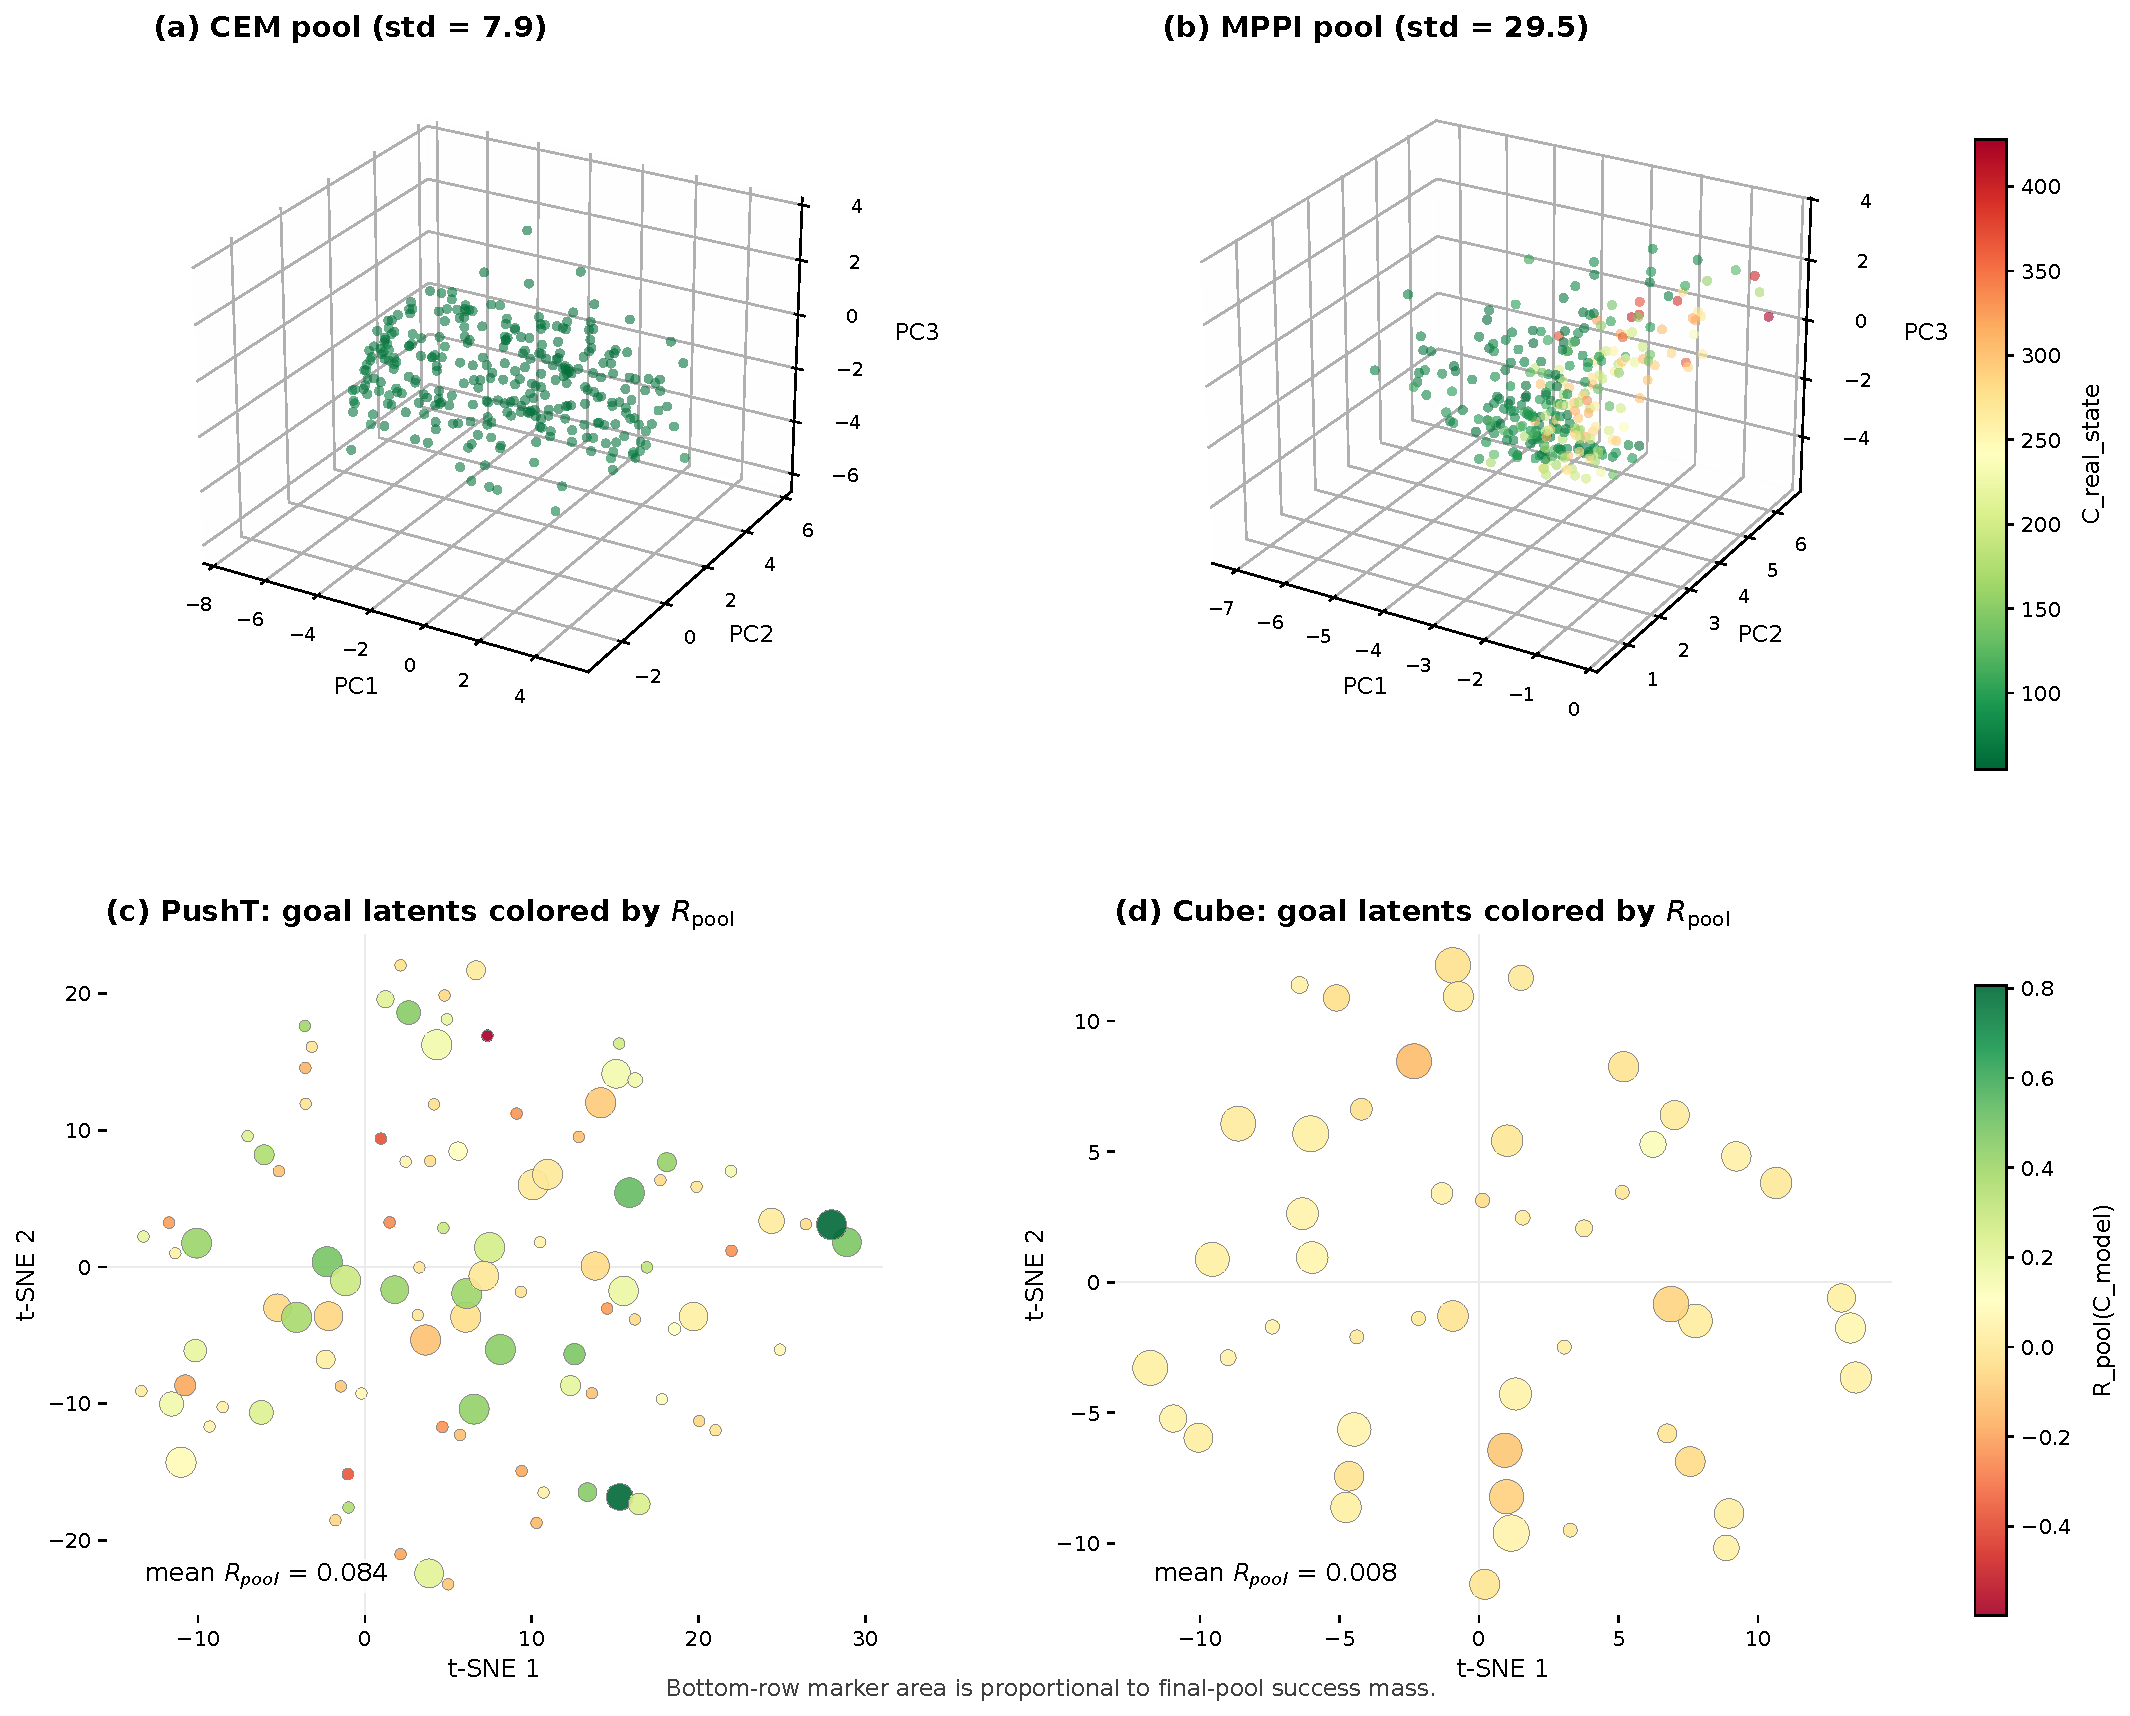
\includegraphics[width=\textwidth]{figures/fig6_spatial.pdf}
\caption{Spatial diagnostics for optimizer and cross-environment analysis. \textbf{(a,b)}~CEM compresses the candidate pool into a tight latent-space cluster ($\mathrm{std}=\mathbf{7.9}$), while MPPI with soft weighting preserves 3.7$\times$ more physical diversity ($\mathrm{std}=\mathbf{29.5}$); both pools are shown for pair~61 under the same PCA projection, colored by physical cost $C_{\text{real\_state}}$. \textbf{(c,d)}~Goal-latent t-SNE maps for PushT (100 pairs) and OGBench-Cube (50 pairs), colored by $\Rpool(\Cmodel)$ with marker area proportional to pool success mass. Near-zero $\Rpool$ (yellow/red) dominates both environments, confirming cross-environment consistency of endpoint-planning decoupling.}
\label{fig:spatial_evidence}
\end{figure*}

The MPPI comparison therefore serves as an optimizer-dependence sanity check rather than a precise attribution of the gap. Soft weighting preserves more physical pool diversity (3.7$\times$) and modestly improves $\Rpool(\Cmodel)$, but it does not close the endpoint-pool gap. Using $\Rendpoint=0.495$ at $m=192$ as the reference, MPPI retains only about 39\% of the endpoint ranking signal ($0.194/0.495$). The wide paired-bootstrap confidence interval for the CEM-specific fraction ($[-16,48]\%$) precludes a precise decomposition. The qualitative finding is that most of the decoupling persists under soft weighting.

\subsection{Cross-Model Validation: DINO-WM}
\label{sec:dinowm}

DINO-WM \citep{zhou2024dinowm} uses a frozen DINOv2 ViT-S/14 encoder with a ViT-style causal Transformer predictor. Its terminal cost combines MSE over predicted visual patch features with proprioceptive MSE, optimized by CEM with the same 300/30/30 configuration as LeWM.

\begin{table}[t]
\centering
\caption{Cross-model comparison of pool-level ranking on PushT. Both models exhibit near-zero $R_{\text{pool}}$ despite different architectures, encoders, and cost functions. DINO-WM results use 29 of the same 30 Track~A pairs (one pair excluded due to scoring timeout).}
\label{tab:cross_model}
\begin{tabular}{lcc}
\toprule
Metric & LeWM & DINO-WM \\
\midrule
Encoder & Learned JEPA & Frozen DINOv2 ViT-S/14 \\
Predictor & Linear/MLP & ViT causal Transformer \\
Terminal cost & $\|z - z_g\|^2$ & MSE patches + $\alpha$ MSE proprio \\
$R_{\text{pool}}(C_{\text{model}})$ & 0.084 & 0.002 \\
Pool $C_{\text{model}}$ std & 2.11 & 0.063 \\
Pool $C_{\text{real}}$ std & 7.84 & 60.6 \\
Planning success & 29.6\% & 3.4\% \\
Selection regret & 19.2 & 128.6 \\
\bottomrule
\end{tabular}
\end{table}

Both models exhibit near-zero pool-level ranking ($R_{\text{pool}} \approx 0$) with severe cost compression (pool $C_{\text{model}}$ standard deviation orders of magnitude below pool $C_{\text{real}}$ standard deviation), confirming that the endpoint-planning decoupling is not specific to LeWM's learned encoder or Euclidean cost. DINO-WM's frozen DINOv2 features and patch-level MSE cost produce the same structural failure: the terminal cost compresses in the CEM-converged region and loses local order preservation. Notably, DINO-WM also shows weak endpoint ranking ($R_{\text{endpoint}} \approx 0.003$), suggesting that the frozen visual encoder may lack task-relevant structure even globally, compounding the local pool-level failure.

These results demonstrate that the three-level diagnostic protocol proposed in this paper applies directly to architecturally distinct latent planners and reveals failure modes that would be invisible under endpoint-only evaluation.
